\section{Evaluation}\label{sec:evaluation}

\subsection{Data inputs}

\textit{We discuss how an attacker can inject arbitrary bytes into receivers.  We measure the effectiveness of this approach by an overshadowing simulation.  We discuss how data can also be inserted through the mailing list}

\subsection{Security audit}
\textit{Table demonstrating which currently-active CVEs are present in the software. A discussion of legacy software and its relation to security}

\subsection{Radio link evaluation}

In order to demonstrate the feasibility of signal injection attacks on EOS downlink systems in a real-world setting, we perform a simulated analysis of the proposed attacks.
We use ``GNU Radio'' to construct a pipeline which simulates a legitimate downlink signal broadcast from the Terra satellite and demodulated by a standard QPSK \textbf{TODO make sure explained} demodulator.
We also simulate an attacker-injected signal added to the legitimate signal and demodulated by the same process.
By varying the gain on the injected signal and measuring the Bit Error Rate (BER) of the decoded bytes, we can assess the transmission power required for the attack to succeed.
An overview of the pipeline is shown in Figure~\textbf{TODO}; the source code is also available alongside our other artifacts (\textbf{TODO}).

In order to carry out these simulations with a reasonable degree of confidence that they are an accurate representation of the real world, we established simulation parameters based on known characteristics of the radio systems.
We use the link budget established in~\cite{quinnNew2003} to establish the EIRP \textbf{TODO make sure explained} and free-space path loss of the radio signals transmitted by the Aqua and Terra satellites, as well as the antenna gain for signals within the beam of the receiver, and losses within the signal processing pipeline.
On the attacker's side, we use the following standard formula for computing free-space path loss:
\begin{align}
    \text{FSPL}_{\text{dB}} = 20\log_{10}(d) + 20\log_{10}(f) - 147.55, \label{eq:fspl}
\end{align}
where $d$ is the distance from the receiver in meters, and $f$ is the frequency in hertz.
We use the antenna radiation pattern given by \textbf{TODO} to estimate the out-of-beam gain of the receiver, using a conservative estimate of $-10.0$\,dB.
These key values are summarised in Table~\ref{tab:experimental-values}.

\begin{table}
    \begin{tabular}{lcc}
        \toprule
        & Victim & Attacker \\
        \midrule
        EIRP (dBm) & $44.4$ & $[-100,0)$ \\
        Distance $d$ (km) & $\sim 713$ & $[0, 10)$ \\
        Free-Space Path Loss (dB) & $179.0$ & $\text{FSPL}_{\text{dB}}(d)$ \\
        Amplitude Multiplier $\left(m = 10^{\frac{\text{EIRP}_{\text{dB}}-\text{FSPL}_{\text{dB}}}{20}}\right)$ & $1.86 \cdot 10^{-7}$ & $m$  \\
        Antenna Gain $g_A$ (dB) & $44.1$ & $-10.0$ \\
        Antenna Amplitude Multiplier $\left( m_A = 10^{\frac{g_A}{20}} \right)$ & $160$ & $0.316$ \\
        System Losses (dB) & \textbf{TODO} & \textbf{TODO} \\
        \bottomrule
    \end{tabular}
    \caption{Key values used in overshadowing simulations.}
    \label{tab:experimental-values}
\end{table}

We do not compute the EIRP of the attacker's transmitter, instead taking a range of values between $-100$ and $0$\,dBm.
We also do not accurately model system losses -- since these are consistent between the victim and attacker, we assume their effect on the outcome of the experiment is negligible.
This is verified to be the case by performing the same experiment across a range of noise values and confirming that the result changes by a negligible amount, as seen in Figure~\ref{fig:overshadowing_accuracy}.
For the main experiments, we set the background noise voltage to $1\,$\textmu V and the system noise to $200$\,mV, resulting in a bit error rate below the $5$\% required for the system to function.

\begin{figure}
    \centering
    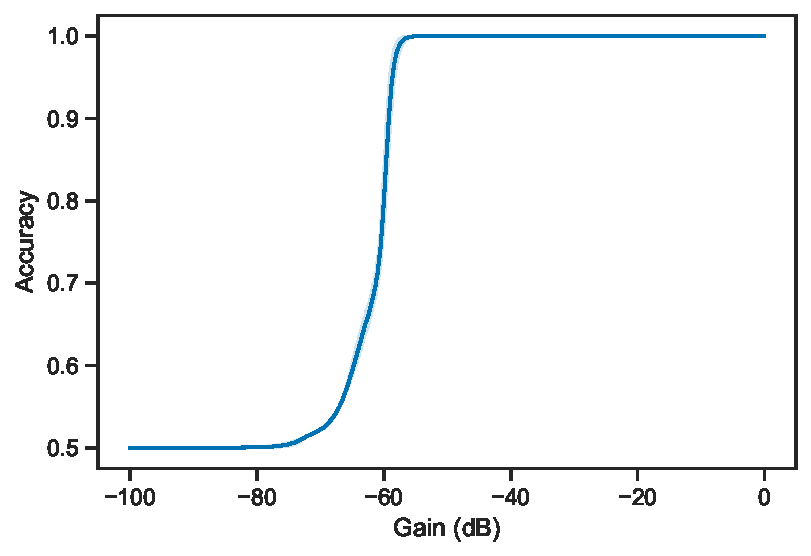
\includegraphics[width=\columnwidth]{diagrams/overshadowing_accuracy.pdf}
    \caption{Proportion of successfully injected bits as the signal strength at the receiver increases. The shaded region represents the range of values under different levels of background and system noise.}
    \label{fig:overshadowing_accuracy}
\end{figure}

The immediate results of our experiment are shown in Figure~\ref{fig:overshadowing_accuracy}, which compares the signal strength at the receiver to the BER of the injected signal.
In order to understand these results in a meaningful sense, we need to instead consider the factors directly controlled by the attacker: the EIRP of the transmitted signal, and the distance between the attacker and the receiver.
We take the EIRP and subtract FSPL (computed from distance using Equation~\ref{eq:fspl}) to get the received signal strength.

\begin{figure}
    \centering
    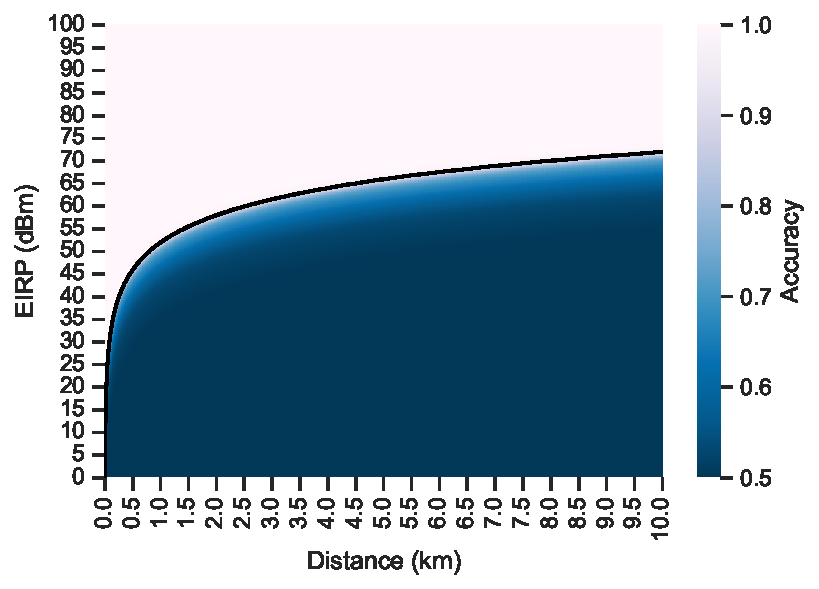
\includegraphics[width=\columnwidth]{diagrams/distance_eirp_heatmap_95.pdf}
    \caption{The accuracy of the injected signal as the attacker varies EIRP and distance from the receiver. The values above which the bit error rate drops below $5$\% are indicated using a line.}
    \label{fig:distance_eirp}
\end{figure}

We see the results in Figure~\ref{fig:distance_eirp}, displaying the BER of the injected signal across a range of EIRPs and distances.
From this result we can understand that the attack is feasible under the assumed threat model -- \textbf{TODO compare to EIRP of COTS equipment, show that it works from around 1km away}


%The proposed evaluation would consist of several stages:

%\begin{itemize}
    %\item A demonstration of calculating the phase cancelling and injecting signal from an arbitrary image
    %\item An evaluation of how often an attacker's receiver station can reliably decode the transmission well enough to perform signal injection
    %\item A demonstration that, given the direct playback transmission, a receiver can successfully synchronise and inject the signal at the right time
    %\item An end-to-end demonstration that the spoofed image can be injected, and then fool the FIRMS forest fire detection algorithm
%\end{itemize}

\begin{figure}
    \centering
    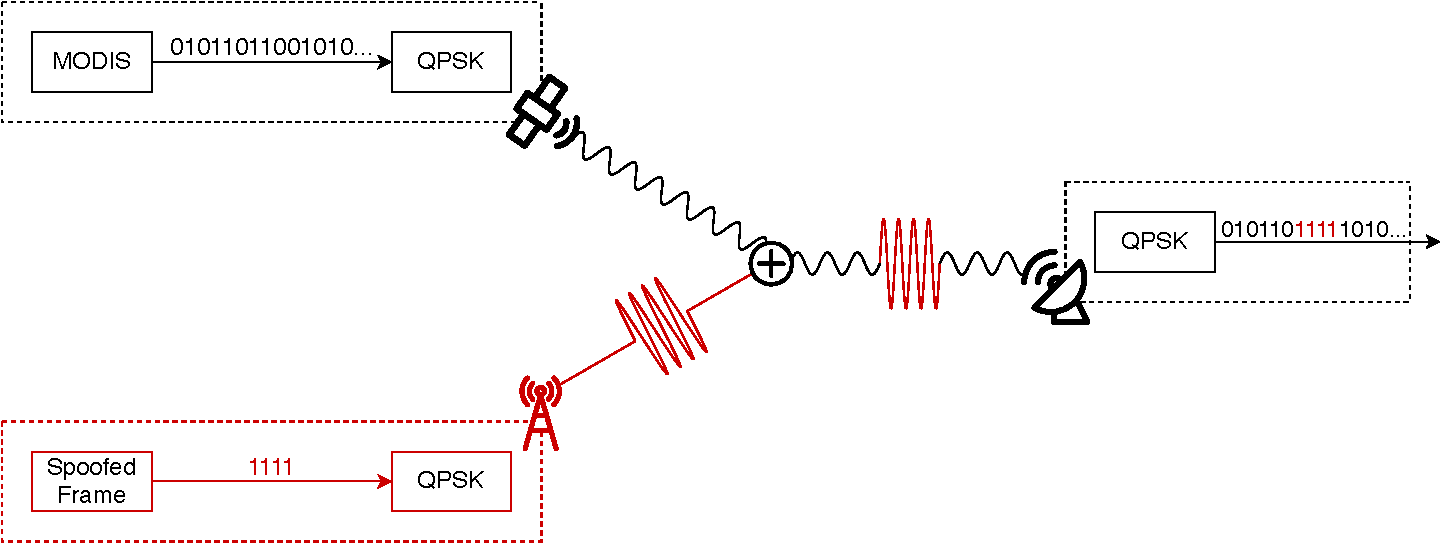
\includegraphics[width=\columnwidth]{diagrams/overshadowing_demo.pdf}
    \caption{Representation of a signal injection attack through overshadowing.}
    \label{fig:overshadowing_demo}
\end{figure}

\begin{comment}
In order to demonstrate the feasibility of signal injection through overshadowing in a real-world setting, we construct an end-to-end software pipeline to demonstrate the attack.
This pipeline, built using ``GNU Radio'', encodes the victim's signal using the QPSK modulation pipeline described in \textbf{TODO}.
An attacker's signal is also encoded and amplified by a specified amount.
At a specified time this signal is injected on top of the victim's signal by adding the samples together, mimicking the behaviour of a radio receiver picking up the two superimposed signals.
A QPSK demodulation pipeline outputs the resulting bytes.
This is illustrated in Fig.~\ref{fig:overshadowing_demo}.

We measure the performance of a given configuration by looking for the frame header bytes in the decoded signal -- these indicate the attacker was successfully able to inject a frame.
For each configuration we repeat the attack 1024 times to get an overall success rate for that configuration.
We measure success rate for varying levels of background noise, and power of the attacker's signal.
Signal-to-noise ratio (SNR) is computed from the victim signal using the following:

\begin{equation}
\label{eq:snr}
    \text{SNR} = \frac{\text{signal amplitude}^2}{\text{noise amplitude}^2}
\end{equation}

\begin{figure*}
    \centering
    \begin{subfigure}{0.95\columnwidth}
        \centering
        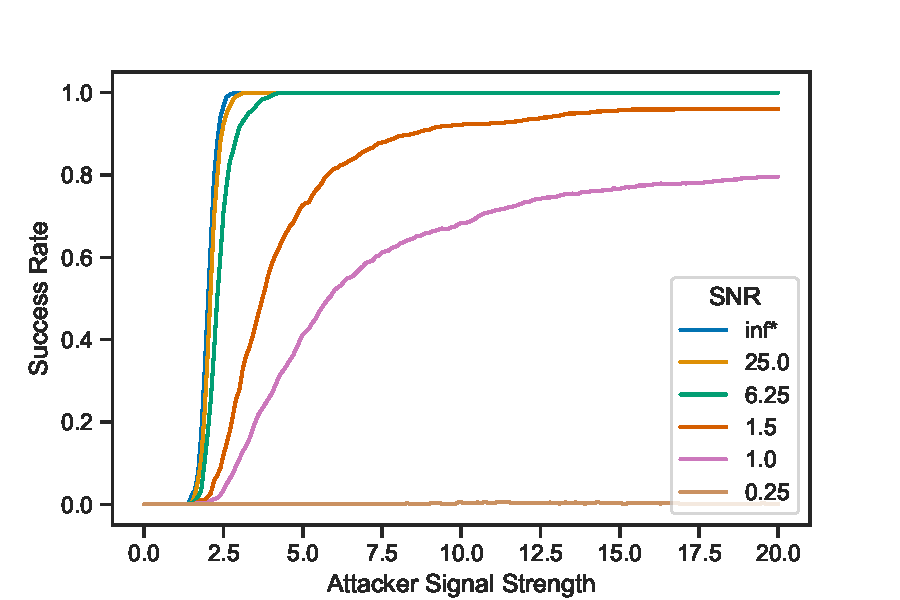
\includegraphics[width=\columnwidth]{diagrams/attack_strength.pdf}
        \caption{Success rate as signal strength increases, for a range of SNRs.\\\footnotesize{\normalfont{*no noise on channel}}}
        \label{fig:attack_strength}
    \end{subfigure}
    \hfill
    \begin{subfigure}{0.95\columnwidth}
        \centering
        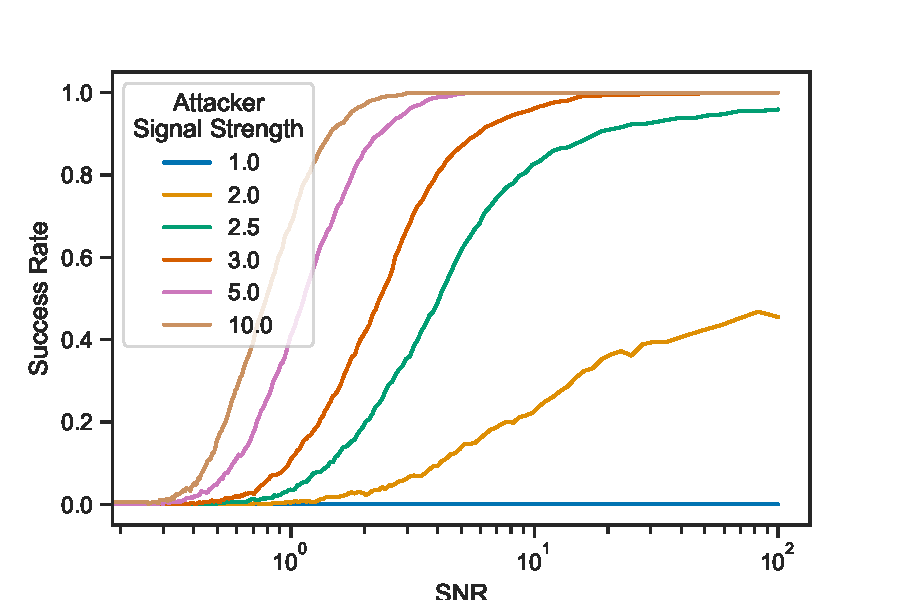
\includegraphics[width=\columnwidth]{diagrams/attack_snr.pdf}
        \caption{Success rate as SNR increases, for a range of signal strength values.}
        \label{fig:attack_snr}
    \end{subfigure}
    \caption{Success rate of signal overshadowing. Signal strength given as a multiple of victim signal strength.}
\end{figure*}


Fig.~\ref{fig:attack_strength} illustrates the success rate of the attack as we increase the power of the attacker's signal for a range of background noise levels.
Similarly, Fig~\ref{fig:attack_snr} shows the success rate of the attack for various attacker power levels, as we vary the noise on the receiver.
It is clear that with low to moderate levels of noise the success rate of the attack eventually reaches 100\%.
By measuring the noise level at the receiver and consulting this figure, the attacker can derive the minimum transmission power required (relative to the victim signal) to overshadow the signal with a maximal success rate.
When noise is low, the signal needs to be roughly $2.5$~times as strong as the victim signal.
Above a certain noise level, the success rate of the attack is unable to reach 100\% -- with this much noise on the channel, not even a legitimate signal is able to get through.
\end{comment}
